\documentclass[11pt,a4paper]{article}

\usepackage[spanish]{babel}
\usepackage[utf8]{inputenc}

\usepackage{amsmath, amssymb}
\usepackage{graphicx}
\usepackage{float}
\usepackage{geometry}
\usepackage{booktabs}
\usepackage{physics}
\usepackage{siunitx}
\usepackage{subcaption}
\usepackage{multirow}
\decimalpoint

\geometry{margin=2.5cm}

\title{Simulación numérica de la órbita del cometa Halley y estudio de la precesión inducida por Júpiter}
\author{Andrés López Serna}
\date{\today}

\begin{document}

\maketitle

\begin{abstract}

En este trabajo se estudia la dinámica orbital del cometa Halley mediante simulaciones numéricas basadas en la ley de gravitación universal.Se estudia en primer lugar la influencia gravitatoria del Sol y se calculan magnitudes orbitales como la energía, el momento angular y los parámetros geométricos de la órbita. Además, se compara la órbita del cometa con la del planeta enano Plutón.

Posteriormente se introduce la presencia de Júpiter con el objetivo de analizar la precesión de la órbita del cometa. Para ello se emplea un método de extrapolación basado en aumentar artificialmente la masa de Júpiter y ajustar linealmente la dependencia de la precesión con dicha masa. Finalmente se compara el comportamiento obtenido con el de otros cuerpos del sistema solar y se analiza un caso adicional correspondiente a la precesión de Mercurio.

\end{abstract}

\section{Introducción}

El estudio de la dinámica orbital de los cuerpos del sistema solar constituye uno de los problemas clásicos de la mecánica celeste. 

En el caso ideal de un problema de dos cuerpos, el movimiento resultante es una órbita cónica, típicamente una elipse cuando la energía total del sistema es negativa. Sin embargo, en el sistema solar real intervienen múltiples cuerpos que generan perturbaciones gravitatorias adicionales, lo que provoca desviaciones respecto al movimiento kepleriano ideal.

El cometa Halley constituye un ejemplo de órbita altamente excéntrica con un largo período orbital de aproximadamente 76 años. Por ese motivo, su trayectoria atraviesa regiones muy diferentes del sistema solar y está afectada por la presencia de diferentes planetas que provocan precesión en su órbita, siendo especialmente relevante la causada por los planetas en particular Júpiter debido a su gran masa.

El objetivo de este trabajo es simular numéricamente la órbita del cometa Halley, analizar sus propiedades dinámicas y estudiar la precesión del perihelio inducida por la interacción gravitatoria con Júpiter. Finalmente, se realizará un estudio similar de la órbita de Mercurio, cuya precesión debida a la presencia de Júpiter es conocida.

\section{Marco teórico}

\subsection{Ley de gravitación universal}

La interacción gravitatoria entre dos masas viene dada por

\begin{equation}
\vec{F} = -\frac{GMm}{r^3}\vec{r}
\end{equation}

donde $G$ es la constante de gravitación universal, $M$ es la masa del Sol, $m$ la masa del cuerpo orbitante y $r$ la distancia entre ambos.

En el caso de un cuerpo de masa despreciable comparada con la del Sol, la aceleración viene dada por

\begin{equation}
\vec{a} = -\frac{GM}{r^3}\vec{r}
\end{equation}

En este trabajo se utilizan unidades astronómicas en las que

\begin{equation}
GM_{\odot} = 4\pi^2
\end{equation}

mientras que la distancia se mide en unidades astronómicas y el tiempo en años.

\subsection{Energía orbital}

Para analizar la energía del cometa Halley, puesto a que lo asumimos de masa despreciable, el estudio se centra en su energía por unidad de masa.

La energía cinética por unidad de masa es

\begin{equation}
E_c/m = \frac{1}{2}v^2
\end{equation}

La energía potencial gravitatoria es

\begin{equation}
E_p/m = -\frac{GM}{r}
\end{equation}

De esta forma, la energía total del sistema por unidad de masa es

\begin{equation}
E_t/m = E_c/m + E_p/m
\end{equation}

En un sistema de dos cuerpos aislado, la energía total se conserva.

\subsection{Momento angular}

El momento angular por unidad de masa en dos dimensiones viene dado por

\begin{equation}
L/m = x v_y - y v_x
\end{equation}

En ausencia de torques externos, esta magnitud permanece constante durante el movimiento orbital.

\subsection{Parámetros orbitales}

Para una órbita elíptica, el semieje mayor se calcula como

\begin{equation}
a = \frac{r_a + r_p}{2}
\end{equation}

donde $r_a$ es el afelio y $r_p$ el perihelio.

La excentricidad orbital es

\begin{equation}
e = \frac{r_a - r_p}{r_a + r_p}
\end{equation}

Finalmente, es relevante tener en cuenta que la tercera ley de Kepler establece

\begin{equation}
T^2 = a^3
\end{equation}

\section{Métodos numéricos}

Las ecuaciones diferenciales que describen el movimiento orbital se resuelven mediante métodos de integración temporal discretos.

\subsection{Método de Euler-Cromer}

Este método actualiza primero la velocidad y posteriormente la posición \ref{giordano}:

\begin{align}
\vec{v}_{i+1} &= \vec{v}_i + \vec{a}_i \Delta t \\
\vec{x}_{i+1} &= \vec{x}_i + \vec{v}_{i+1} \Delta t
\end{align}

Este algoritmo presenta mejor estabilidad que el método de Euler estándar para problemas dinámicos ya que conserva la energía.

\subsection{Método de Verlet}

Para el estudio de la precesión orbital se emplea el algoritmo de Verlet, que posee aún mejores propiedades de conservación de energía:

\begin{align}
\vec{x}_{i+1} = \vec{x}_i + \vec{v}_i\Delta t + \frac{1}{2}\vec{a}_i\Delta t^2
\end{align}

Posteriormente se actualizan las velocidades utilizando el promedio de las aceleraciones debidas a $\vec{x}_{i+1}$ y $\vec{x}_i$.

\subsection{Condiciones iniciales}

Para el cometa Halley se utilizan las siguientes condiciones iniciales en el perihelio:

\begin{itemize}
\item $r_p = 0.59$ UA
\item $v_p = 11.47250862$ UA/año
\end{itemize}

Estas condiciones reproducen el período orbital observado (la velocidad se ha obtenido mediante prueba y error).

\section{Resultados}

\subsection{Órbita del cometa Halley}

Mediante prueba y error, conociendo tanto la distancia en el perihelio como el periodo del cometa, se obtiene que la velocidad en el perihelio es $v_p = 11.47250862$ UA/año. Con este resultado, se realiza la obtención de su órbita mediante el método de Euler-Cromer y se obtiene

\begin{itemize}
\item Afelio: $r_a = 35.294$ UA
\item Velocidad orbital máxima: $v_{máx} = 11.4731$ UA/año $\approx v_p$
\end{itemize}

El afelio obtenido se acerca al observado: $r_{a,obs}=35.1$ UA.

\subsection{Comparación con Plutón}

Se realizó una simulación adicional para Plutón con el objetivo de comparar la geometría orbital.

\begin{figure}[H]
\centering
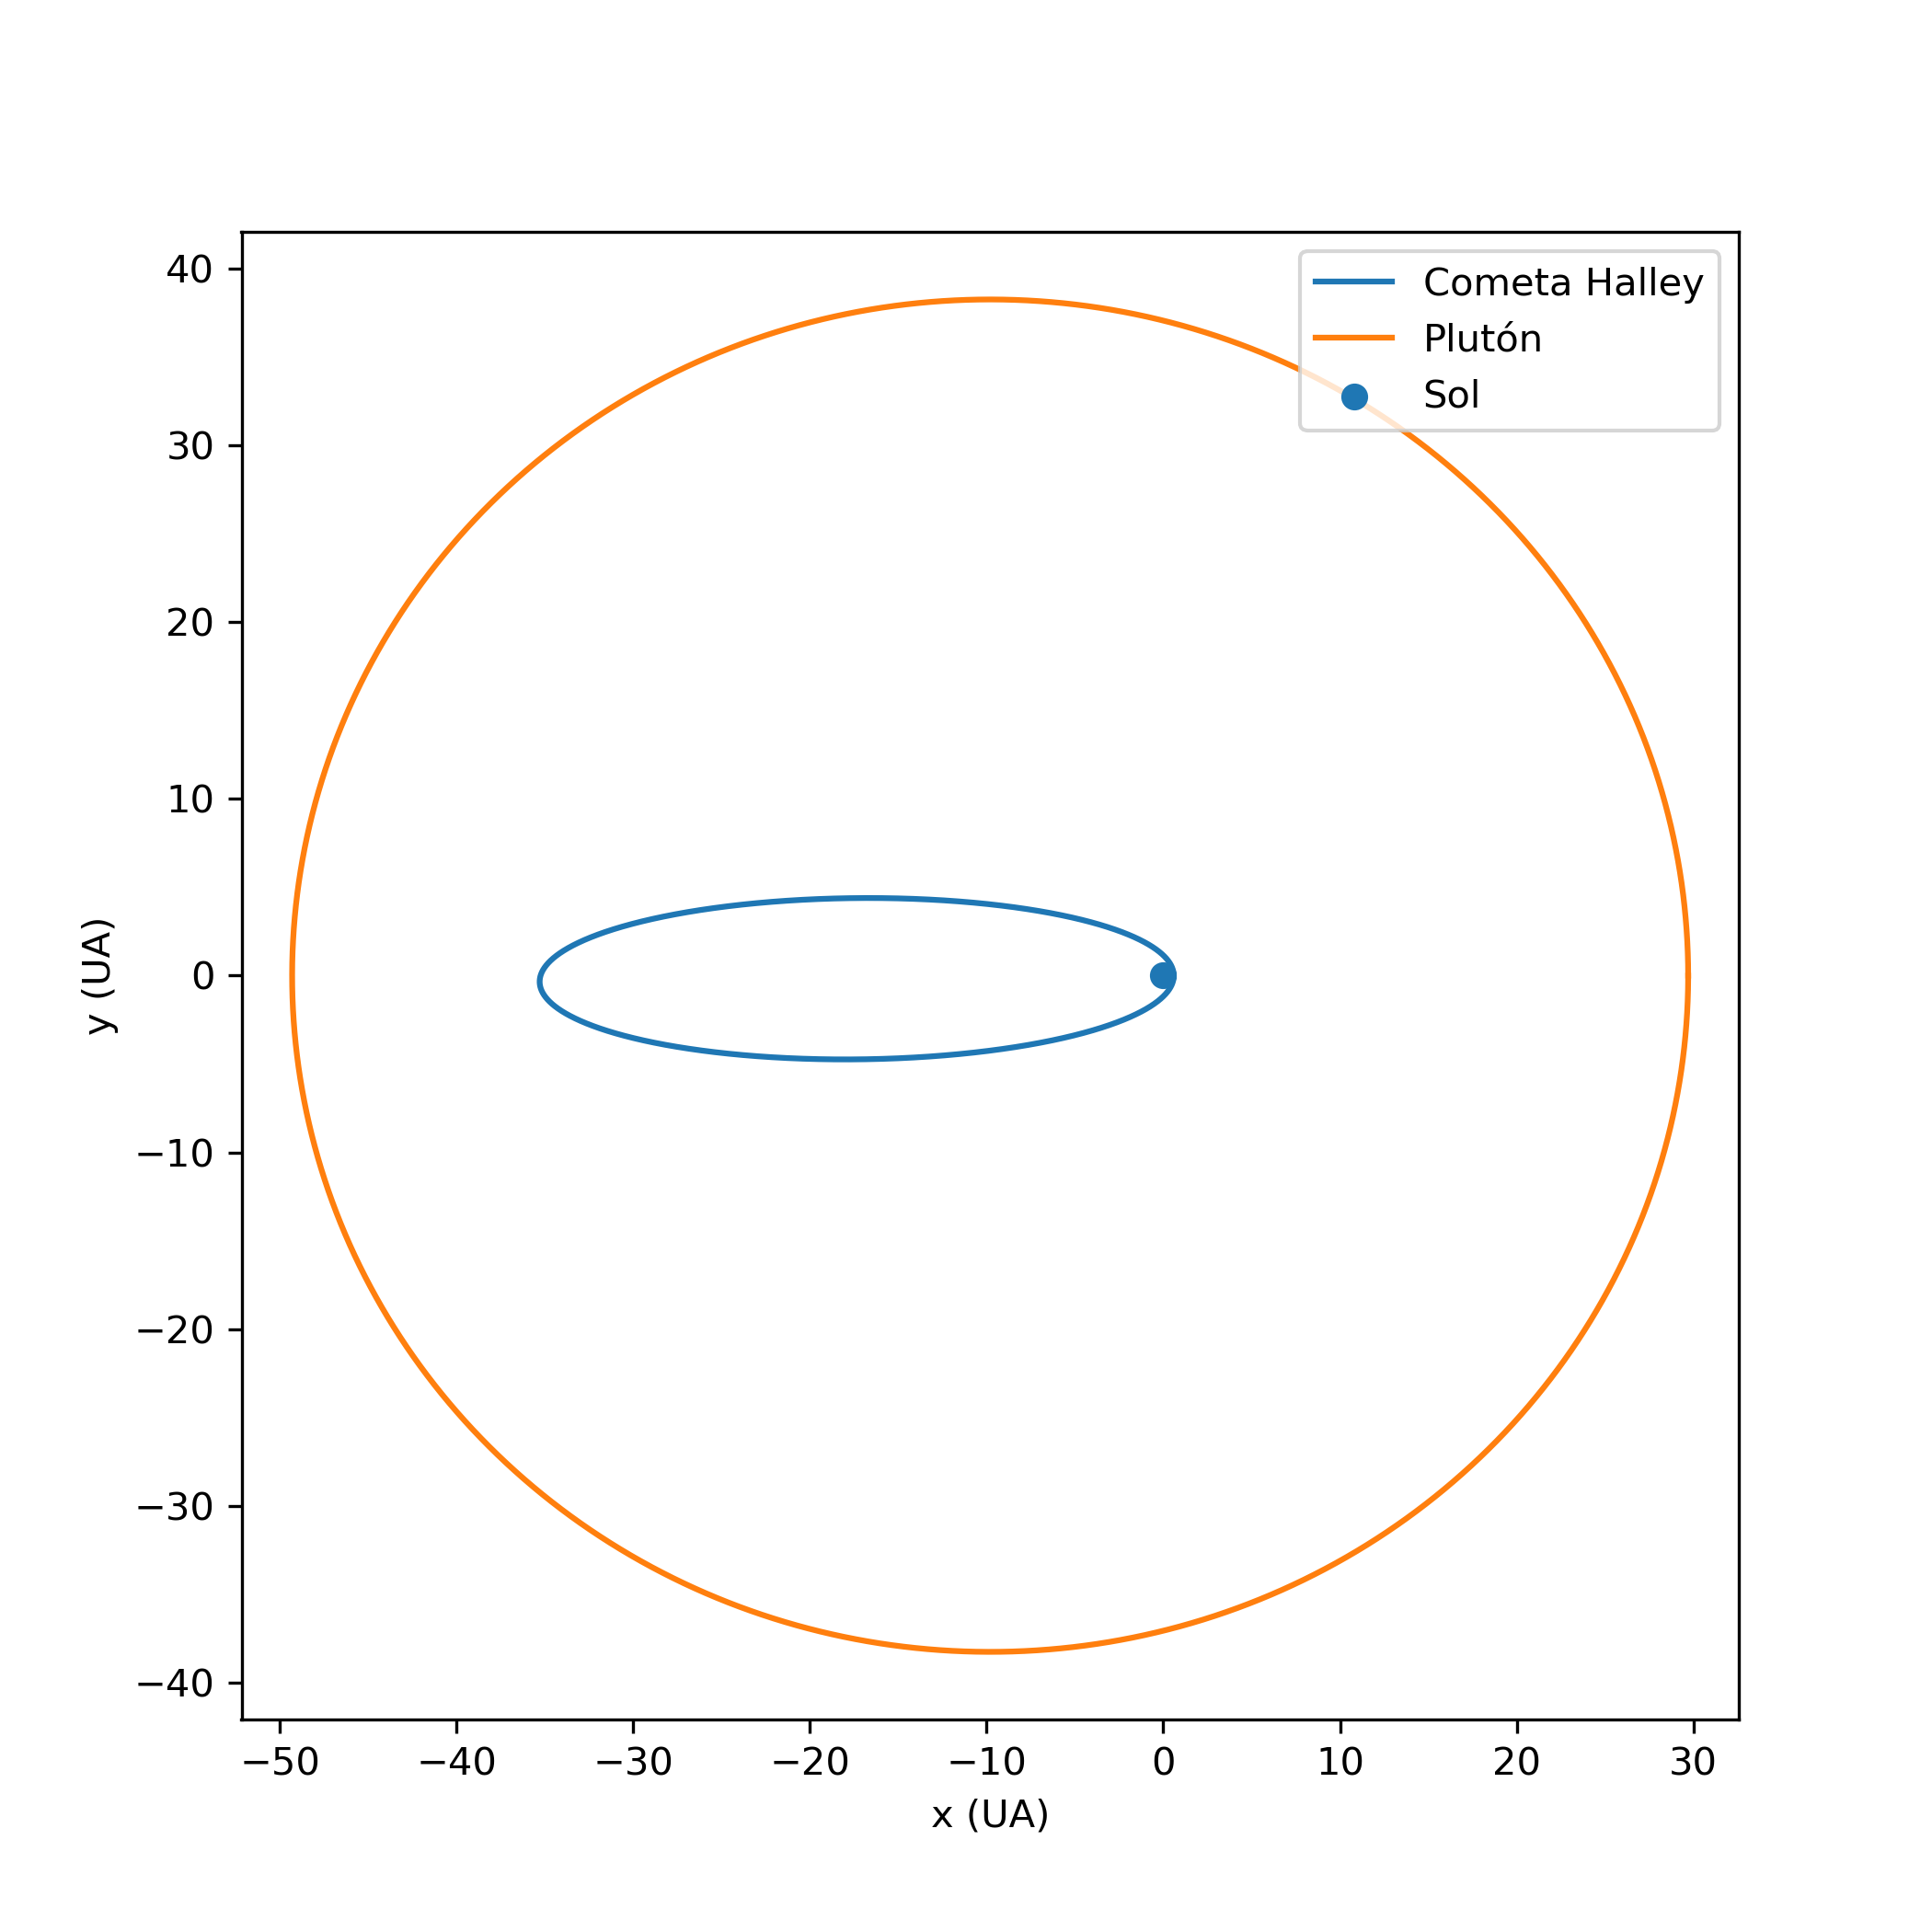
\includegraphics[width=0.5\textwidth]{imagenes/halley_vs_pluton.png}
\caption{Comparación entre las órbitas de Halley y Plutón.}
\label{fig:com}
\end{figure}

En la figura \ref{fig:com} se observa que la órbita de Plutón es significativamente menos excéntrica que la del cometa Halley.

\subsection{Energía y momento angular}

Se obtuvieron también las energías y el momento angular por unidad de masa para el cometa Halley y para Plutón.

\begin{figure}[H]
\centering
\begin{subfigure}[t]{0.49\textwidth}
    \centering
    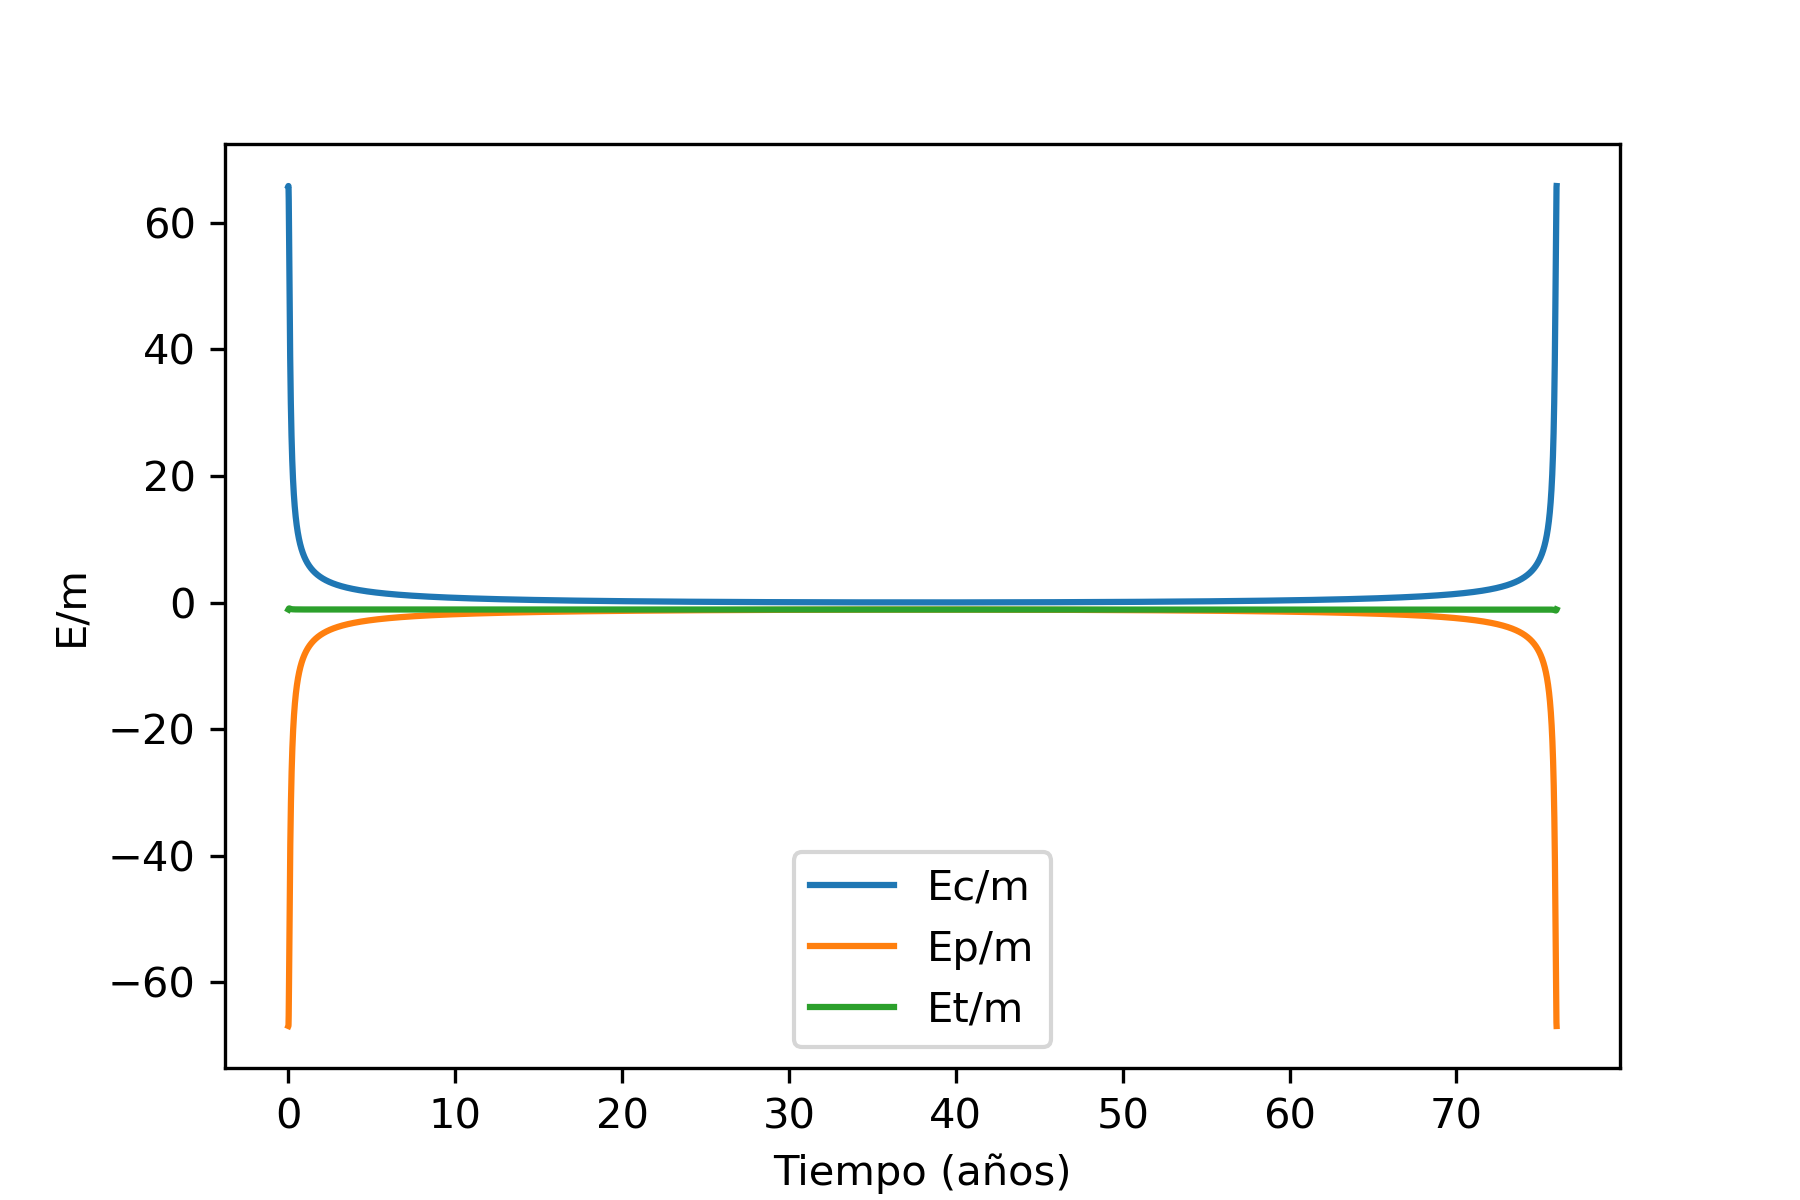
\includegraphics[width=\linewidth]{imagenes/energia_halley.png}
    \caption{Energía orbital del cometa Halley por unidad de masa.}
    \label{fig:energia_halley}
\end{subfigure}
\hfill
\begin{subfigure}[t]{0.49\textwidth}
    \centering
    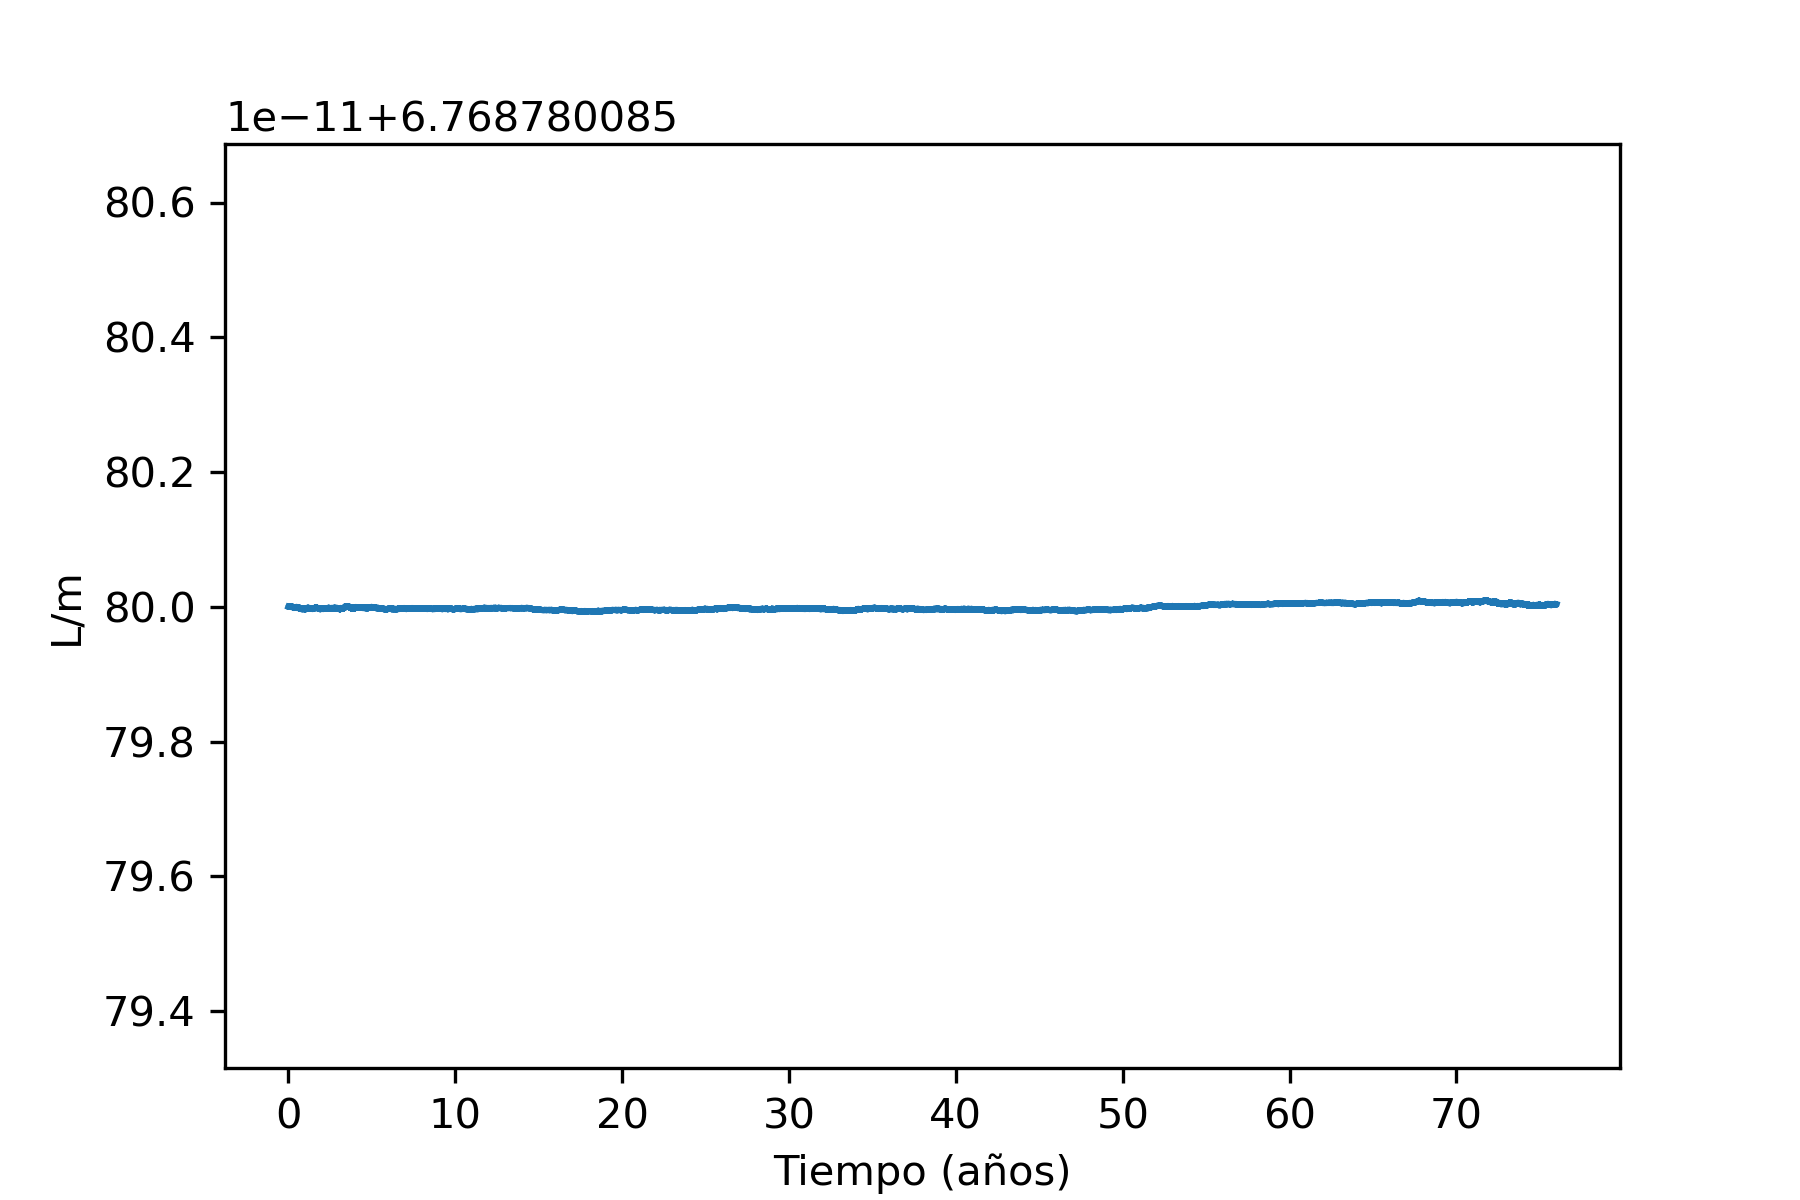
\includegraphics[width=\linewidth]{imagenes/momento_halley.png}
    \caption{Momento angular del cometa Halley por unidad de masa.}
    \label{fig:momento_halley}
\end{subfigure}
\caption{Energía y momento del cometa Halley en función del tiempo para 1 periodo.}
\label{fig:momento_halley}
\end{figure}

\begin{figure}[H]
\centering
\begin{subfigure}[t]{0.49\textwidth}
    \centering
    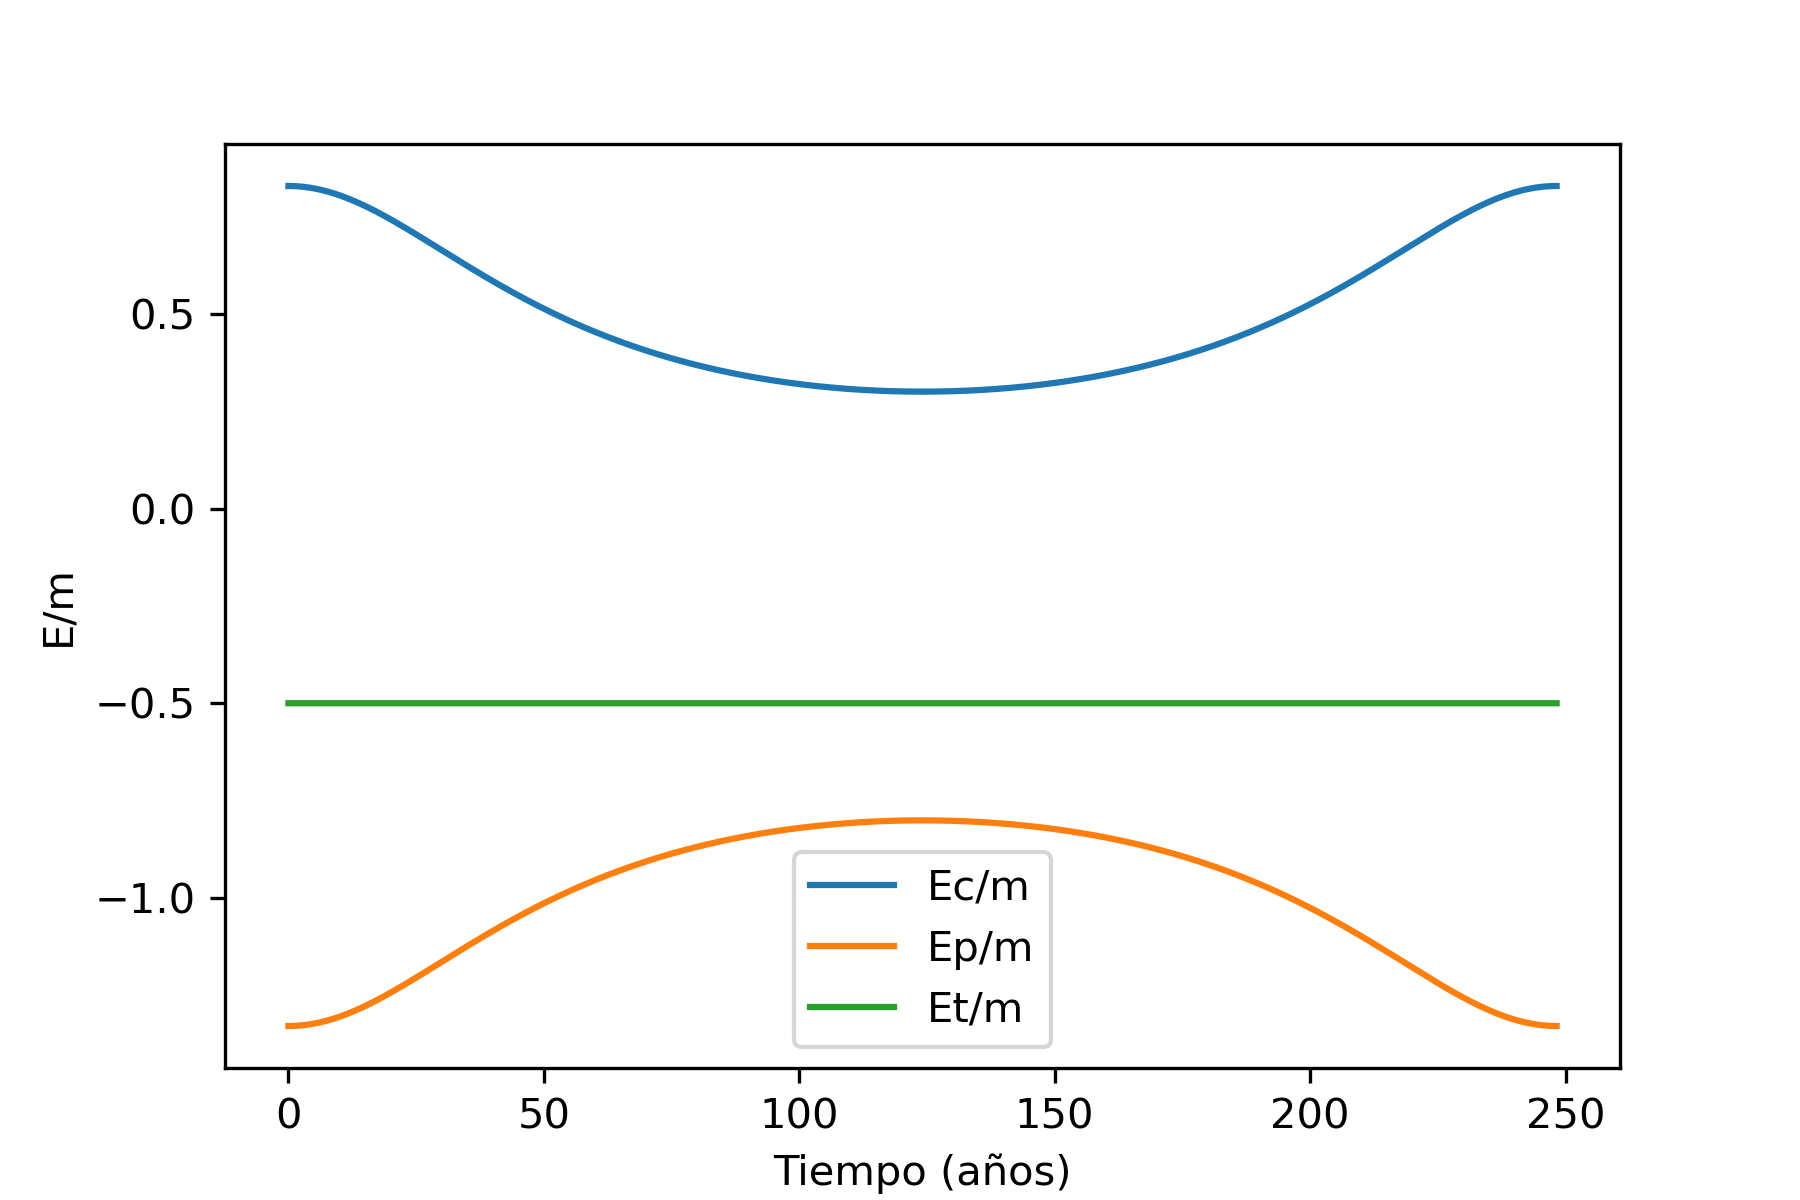
\includegraphics[width=\linewidth]{imagenes/energia_pluton.png}
    \caption{Energía orbital de Plutón por unidad de masa.}
    \label{fig:energia_pluton}
\end{subfigure}
\hfill
\begin{subfigure}[t]{0.49\textwidth}
    \centering
    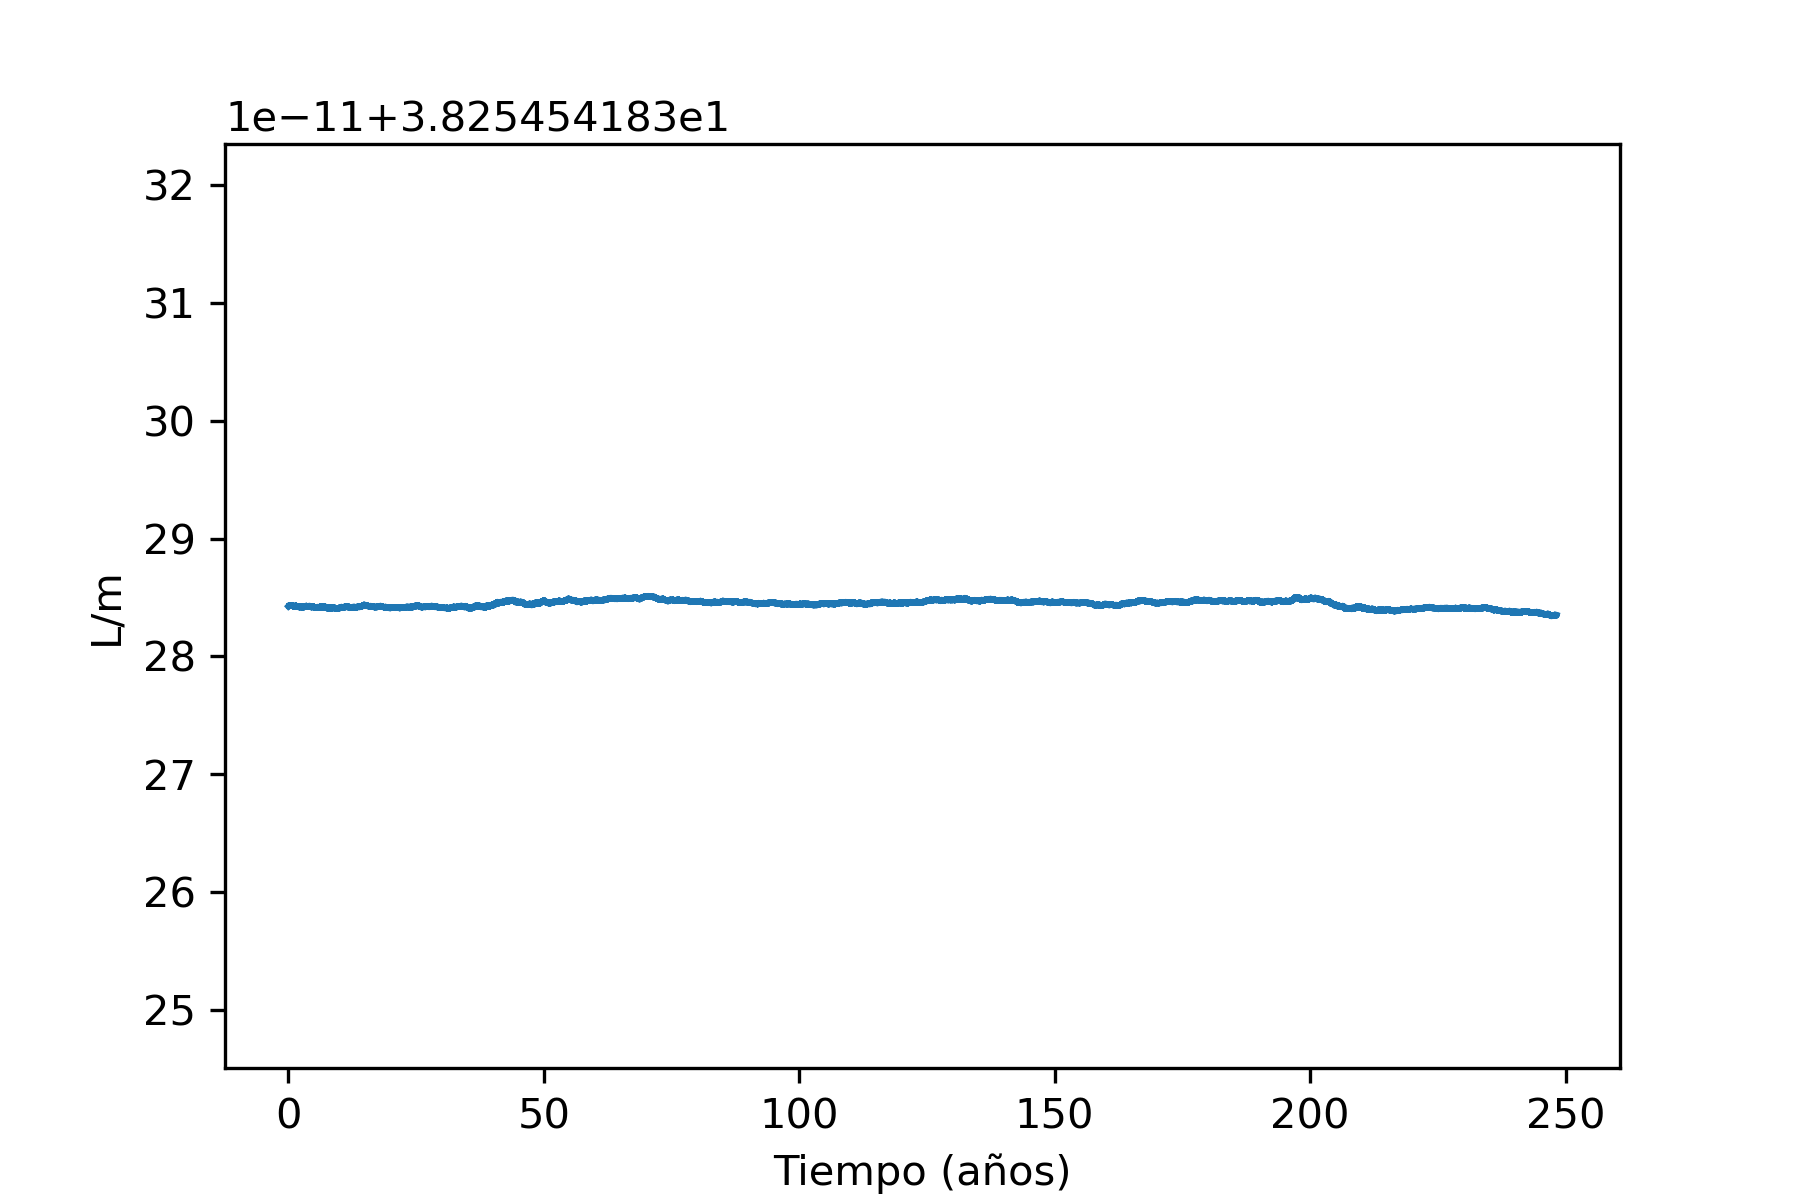
\includegraphics[width=\linewidth]{imagenes/momento_pluton.png}
    \caption{Momento angular de Plutón por unidad de masa.}
    \label{fig:momento_pluton}
\end{subfigure}
\caption{Energía y momento de Plutón en función del tiempo para 1 periodo.}
\label{fig:momento_pluton}
\end{figure}

La energía total y el momento angular (aunque con pequeñas oscilaciones) se mantienen aproximadamente constante durante toda la simulación, lo que indica una correcta estabilidad numérica del algoritmo. Además, se observan los máximos en los módulos de la energía potencial y cinética cuando el cuerpo celeste está cerca del perihelio ($t\approx0$, $t\approx T$). Finalmente, es destacable la anchura de los picos de energía, siendo especialmente finos para el cometa debido a la gran excentricidad de su órbita.

\subsection{Precesión del perihelio}

Al introducir la presencia de Júpiter, aparece una variación progresiva en el ángulo del perihelio.

\begin{figure}[H]
\centering
\begin{subfigure}{0.32\textwidth}
    \centering
    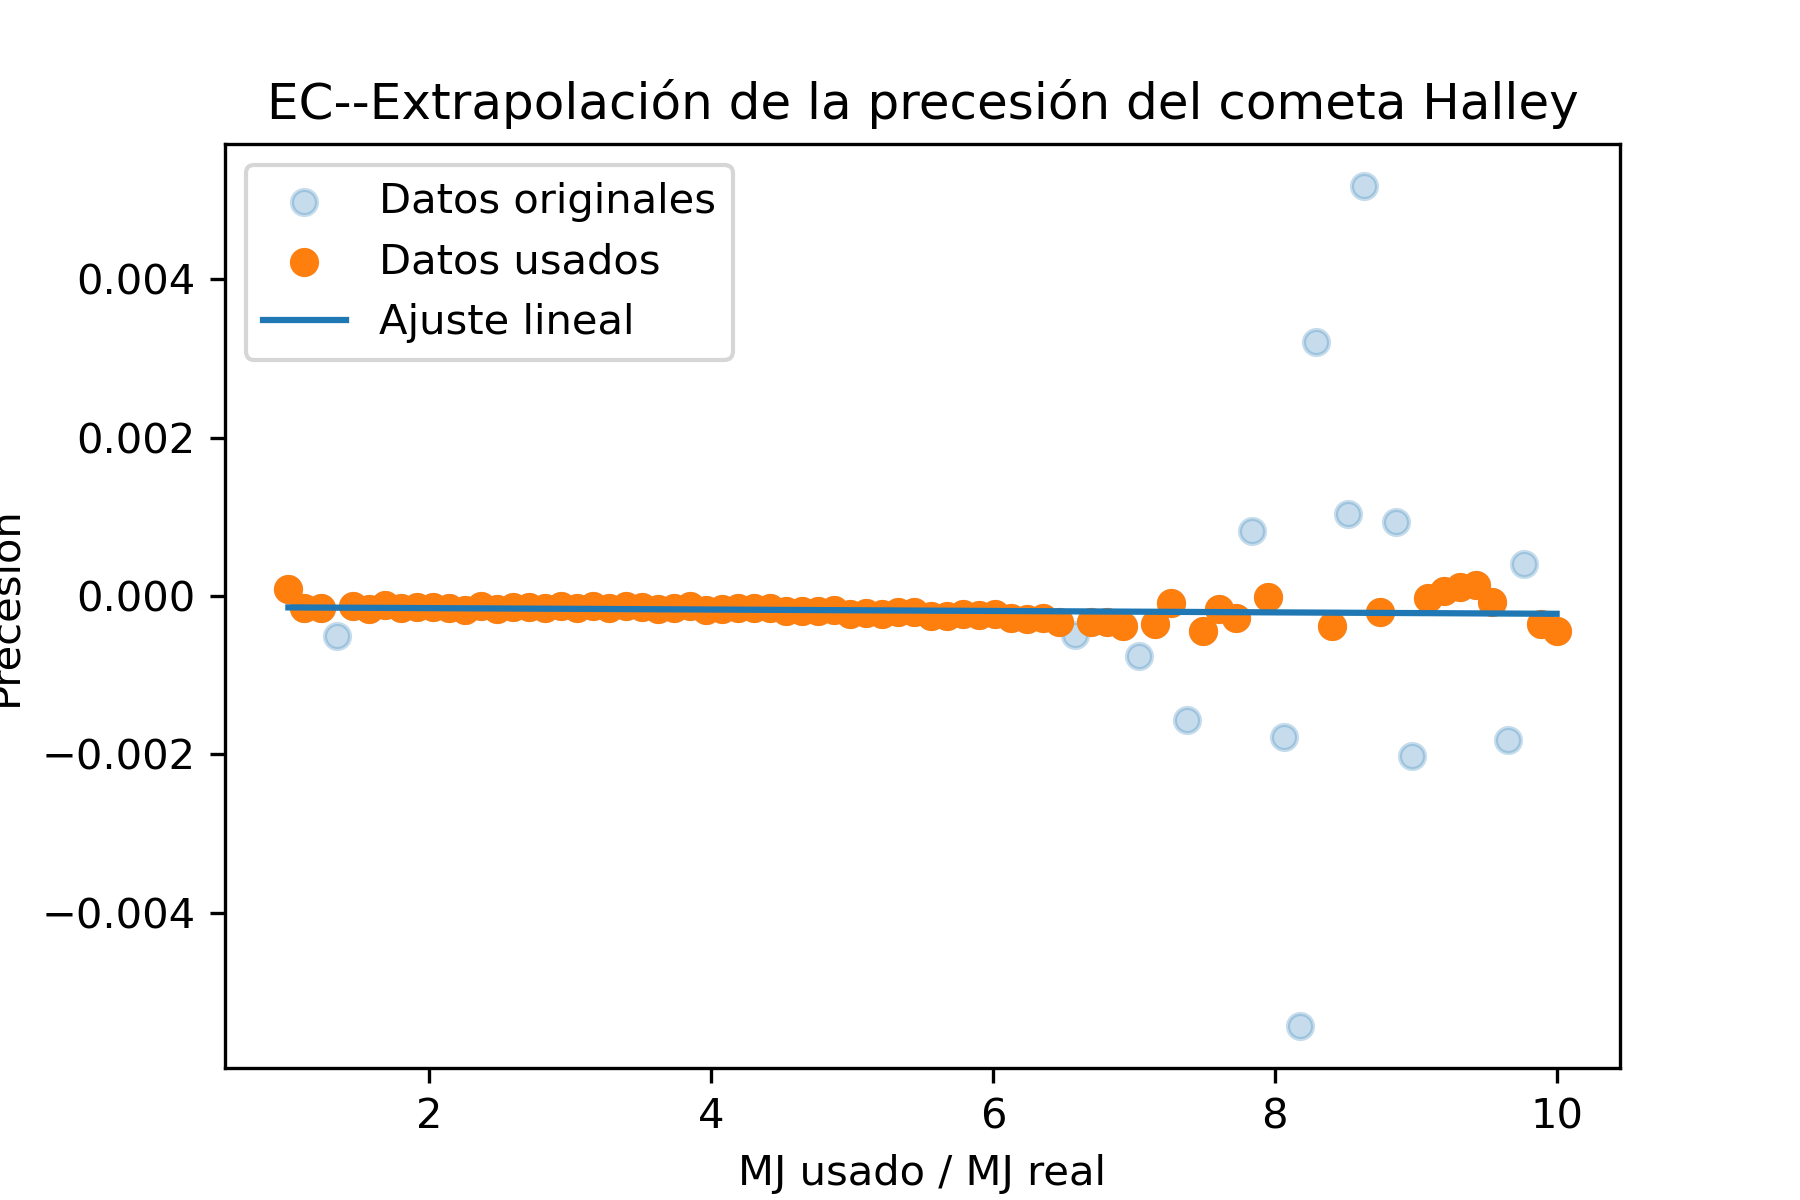
\includegraphics[width=\linewidth]{imagenes/prec_halley_todo_ec.png}
    \caption{Sin filtrar}
\end{subfigure}
\hfill
\begin{subfigure}{0.32\textwidth}
    \centering
    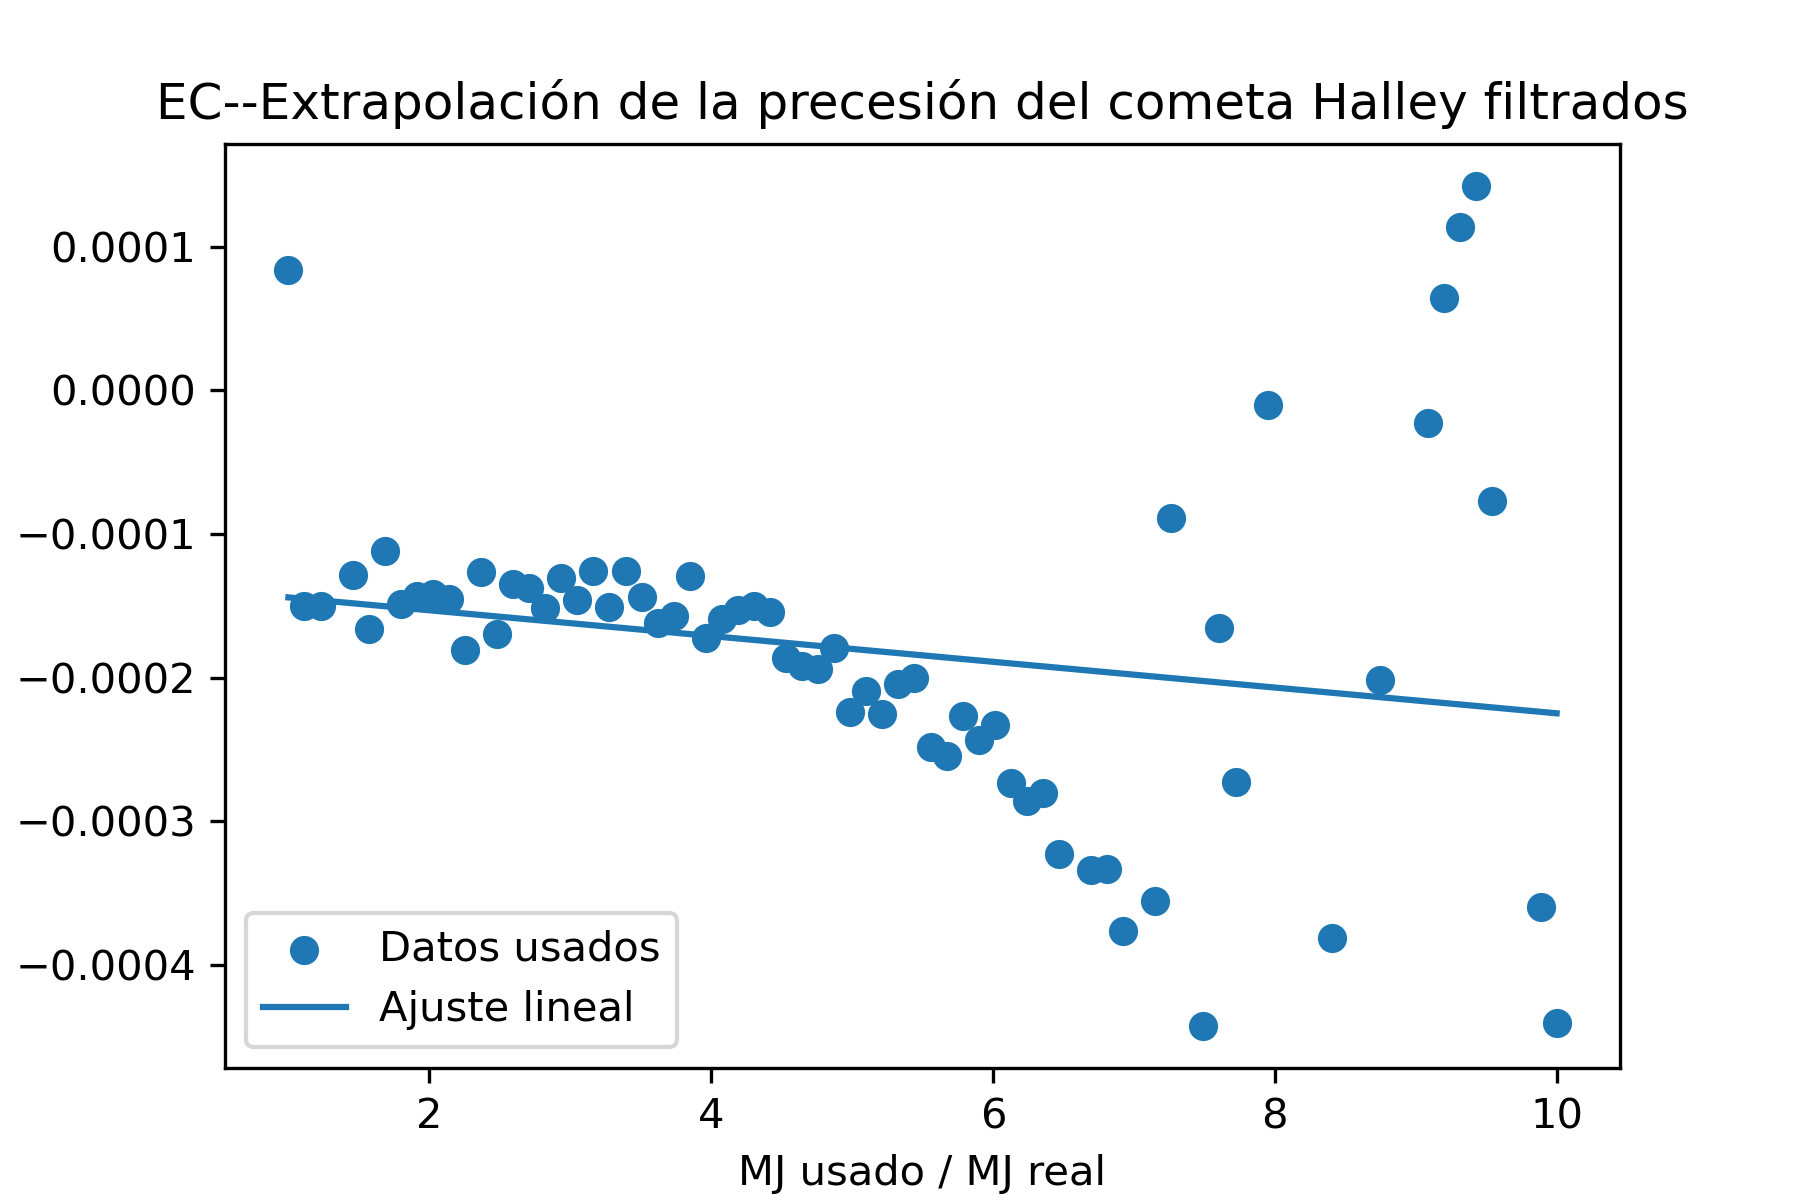
\includegraphics[width=\linewidth]{imagenes/prec_halley_filtrado_ec.png}
    \caption{Tras filtrar}
\end{subfigure}
\hfill
\begin{subfigure}{0.32\textwidth}
    \centering
    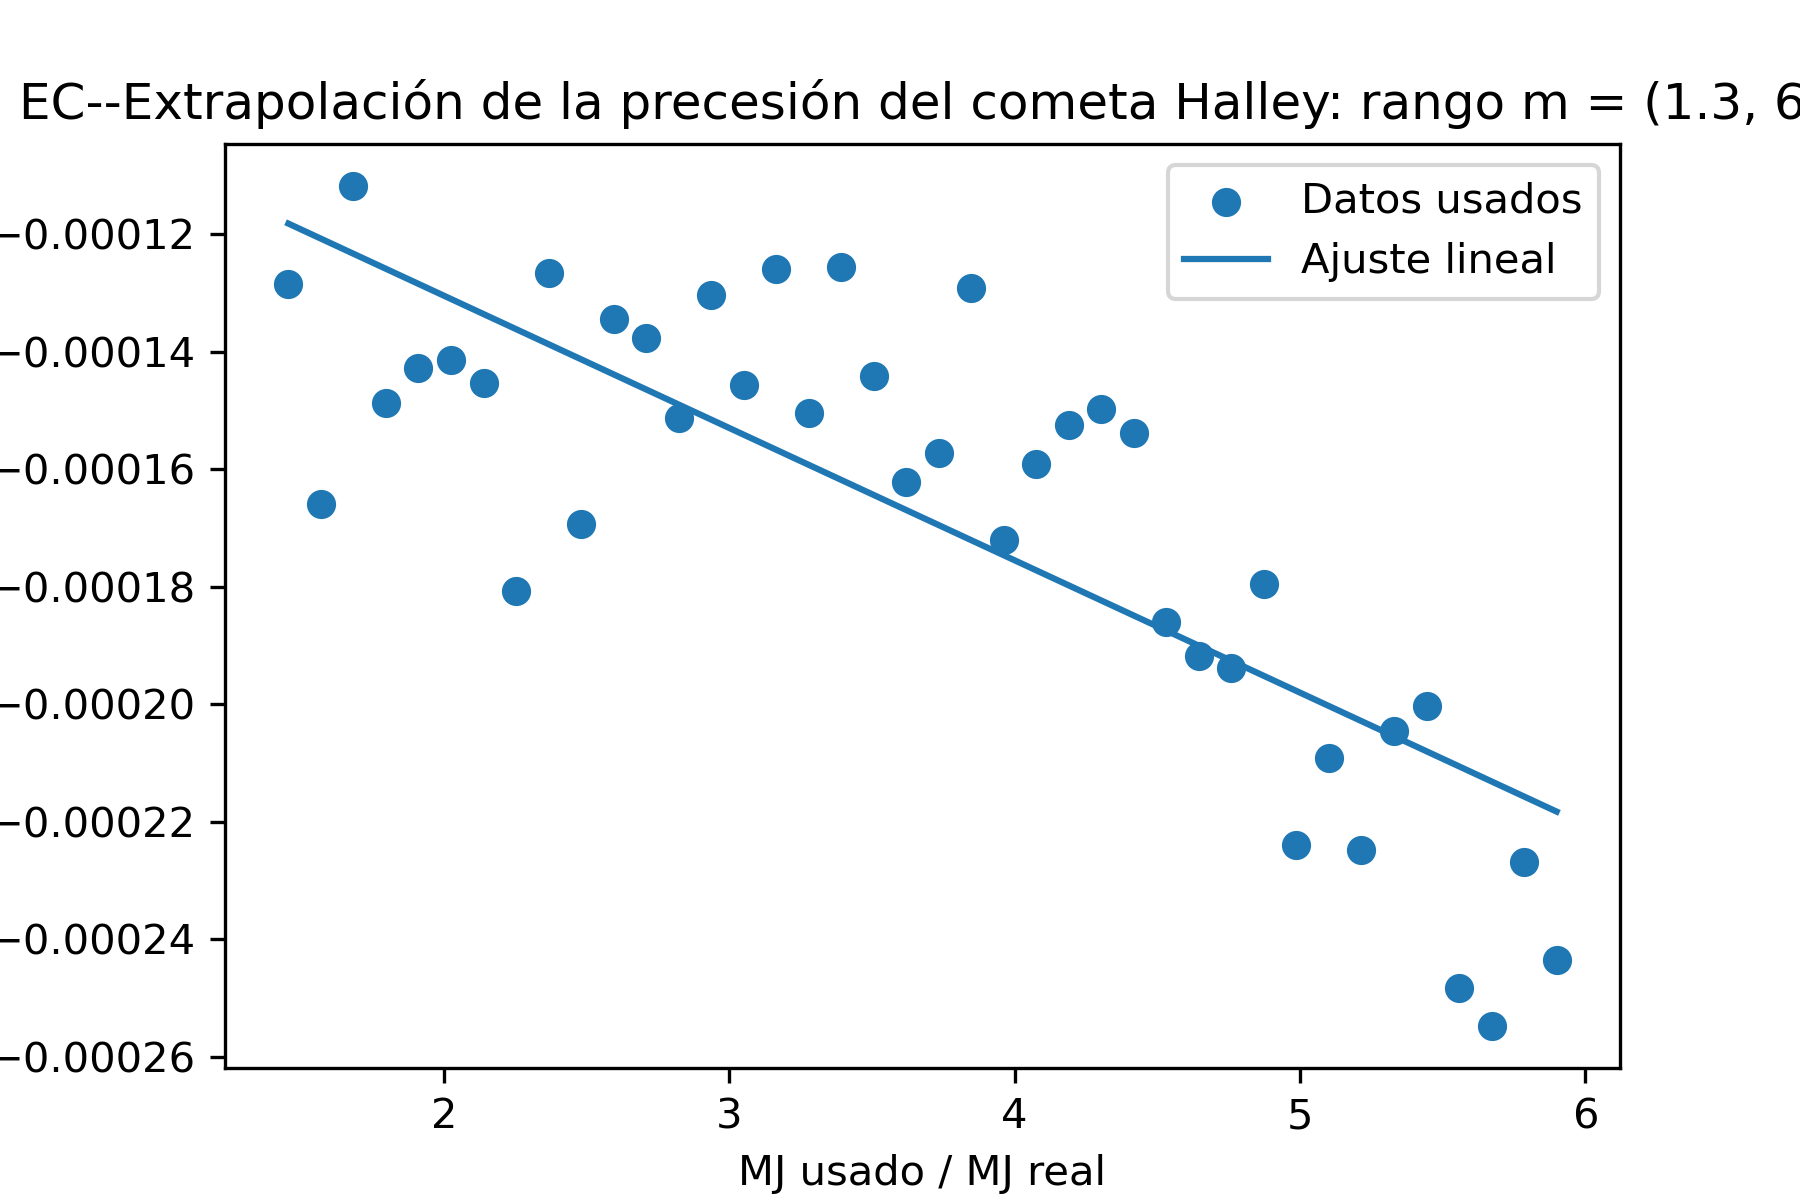
\includegraphics[width=\linewidth]{imagenes/prec_halley_rango_ec.png}
    \caption{$\frac{M_{J,usada}}{M_{J,real}} \in (1.3, 6)$}
\end{subfigure}

\caption{Precesión del perihelio de Halley utilizando Euler-Cromer}
\label{fig:comparacion}
\end{figure}

\begin{figure}[H]
\centering
\begin{subfigure}{0.32\textwidth}
    \centering
    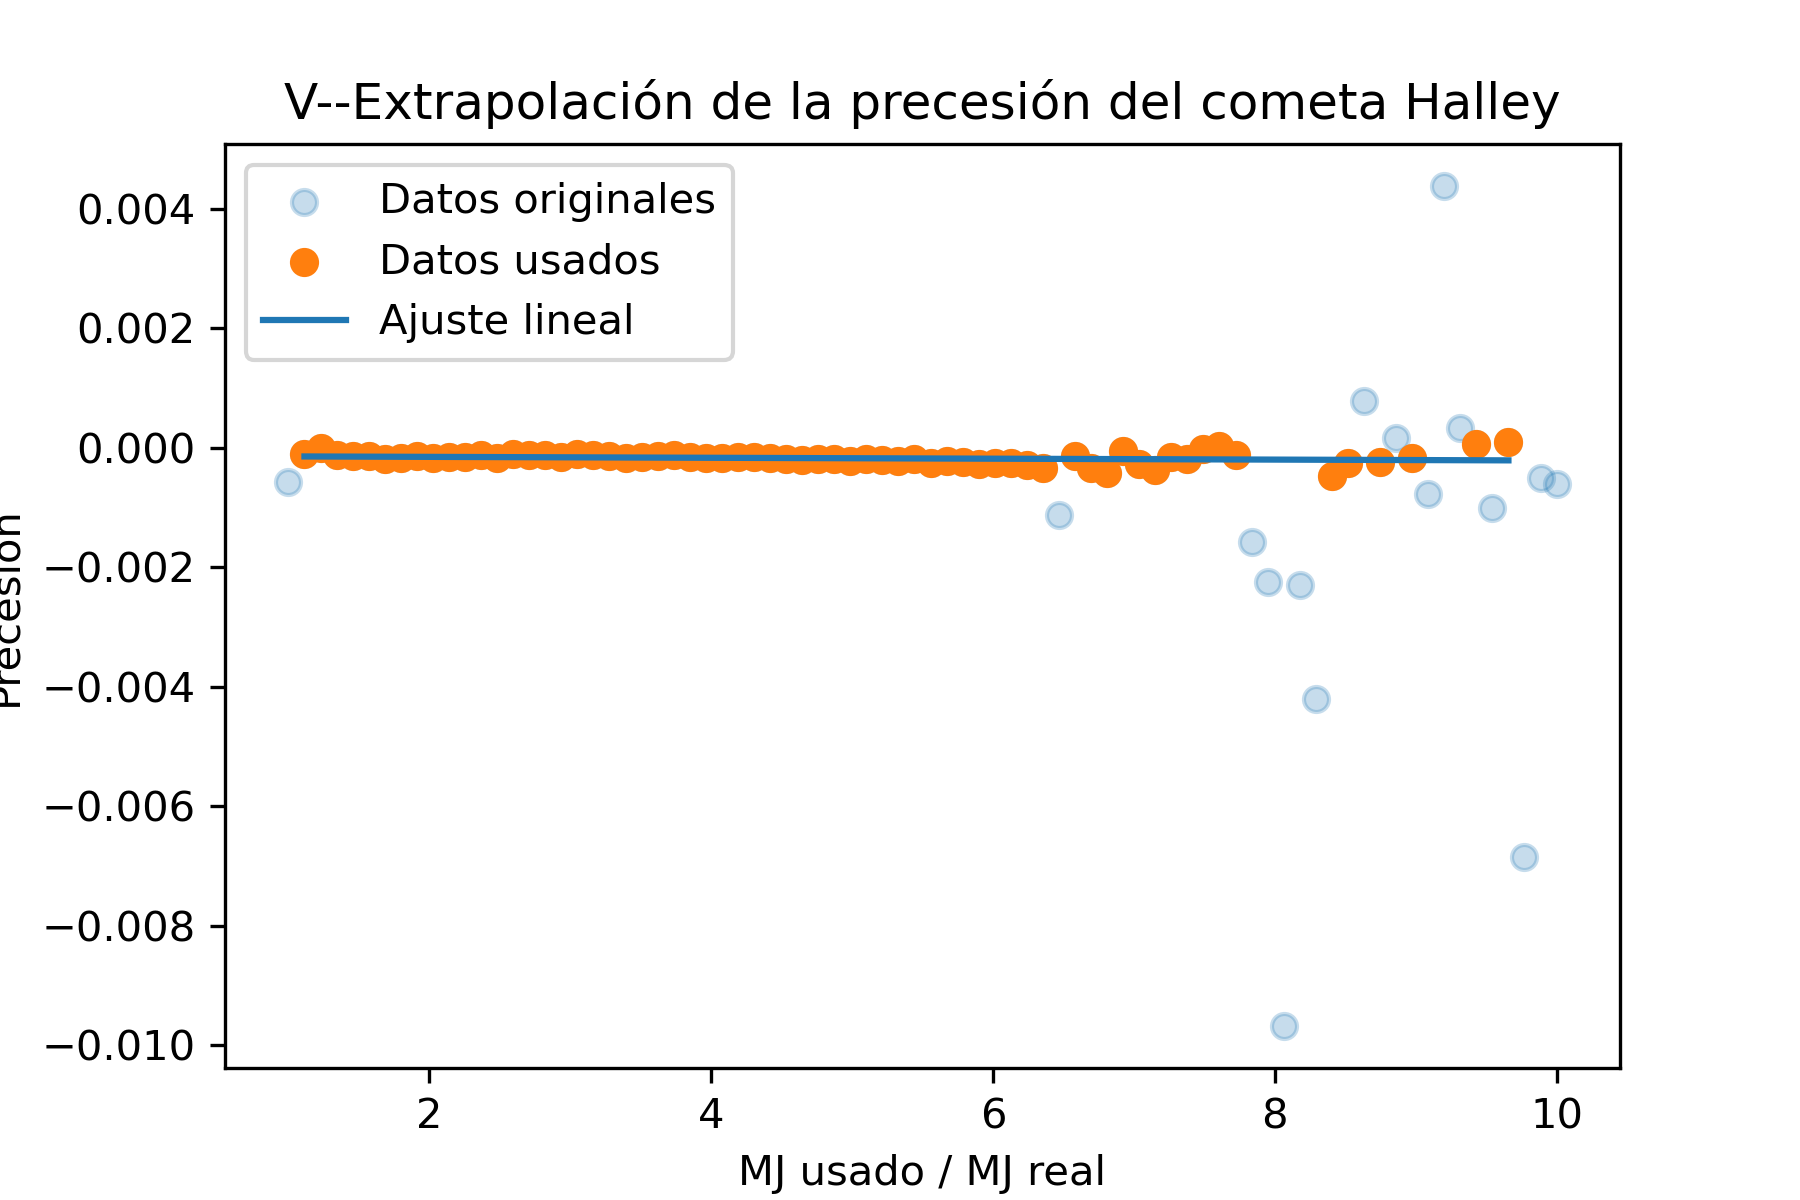
\includegraphics[width=\linewidth]{imagenes/prec_halley_todo_v.png}
    \caption{Sin filtrar}
\end{subfigure}
\hfill
\begin{subfigure}{0.32\textwidth}
    \centering
    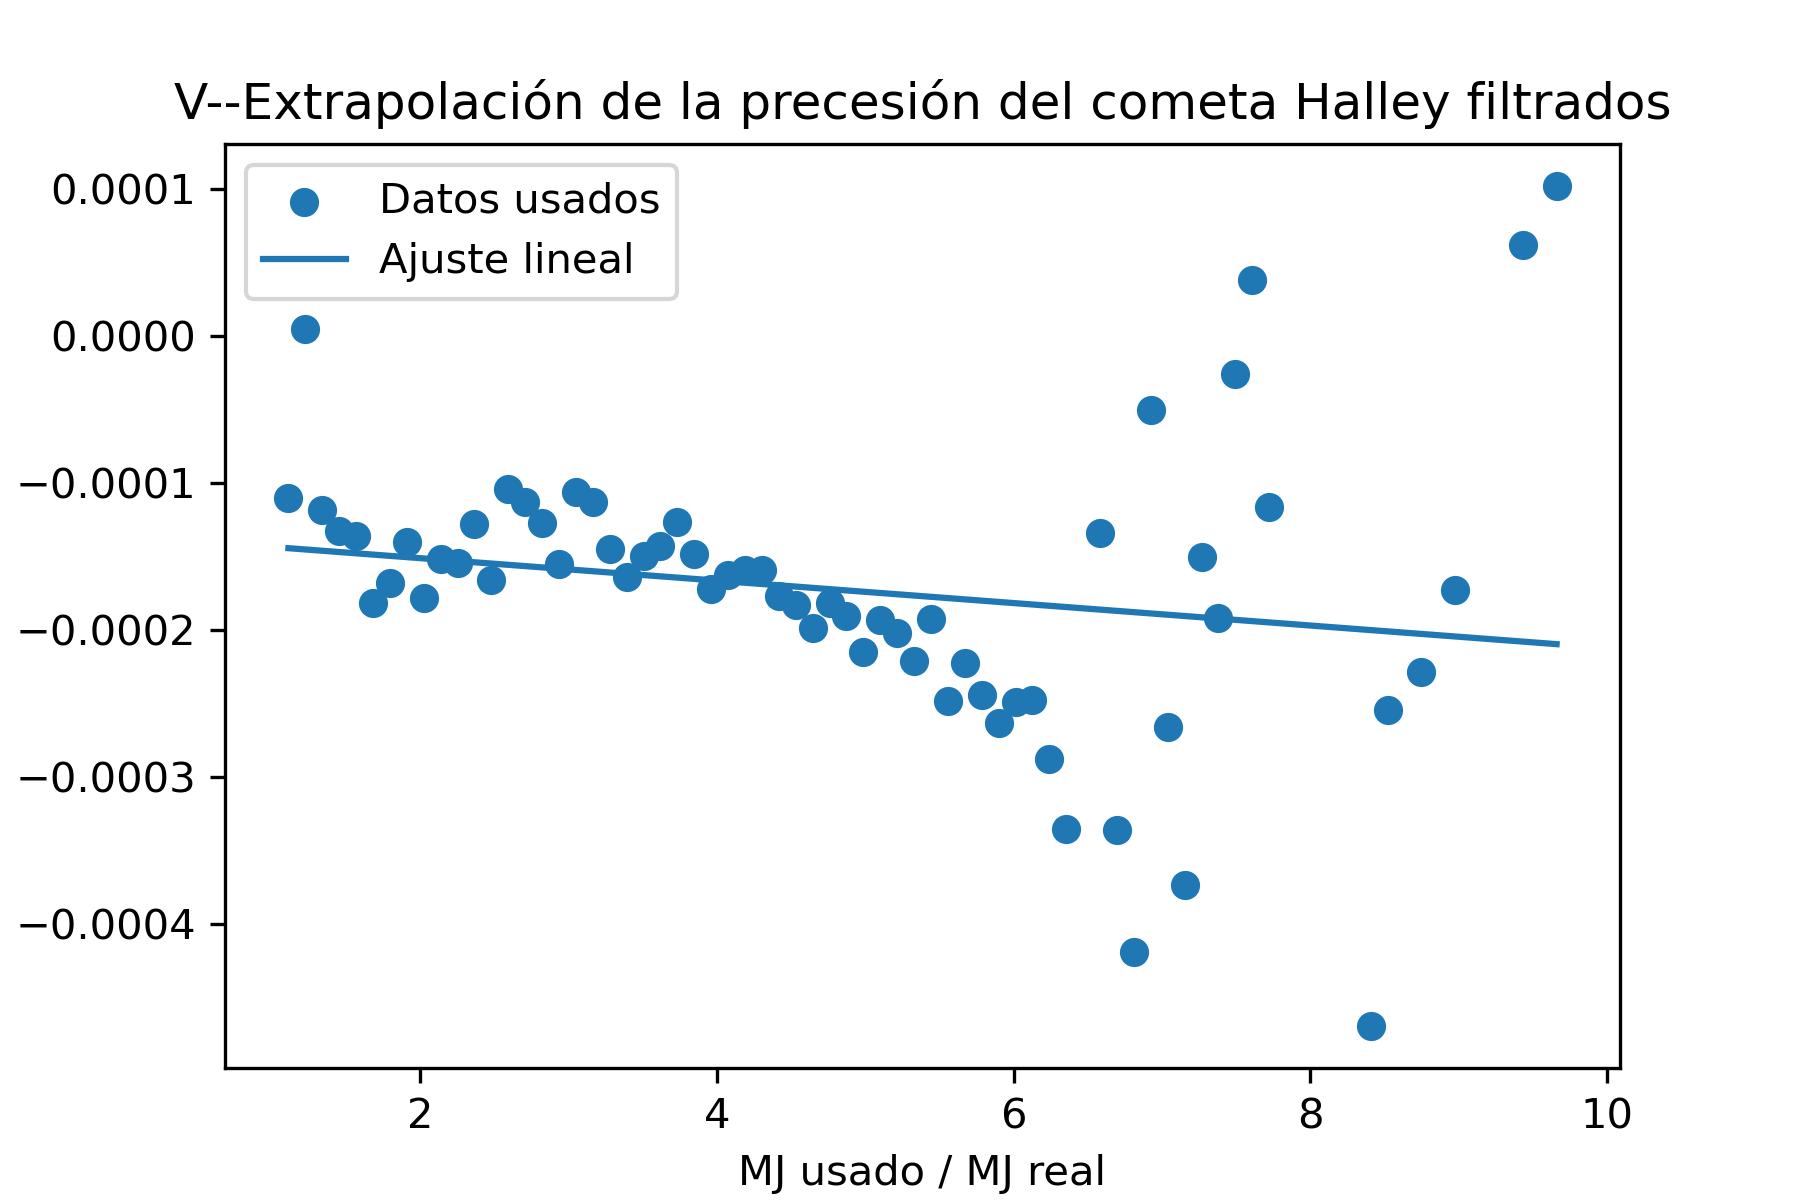
\includegraphics[width=\linewidth]{imagenes/prec_halley_filtrado_v.png}
    \caption{Tras filtrar}
\end{subfigure}
\hfill
\begin{subfigure}{0.32\textwidth}
    \centering
    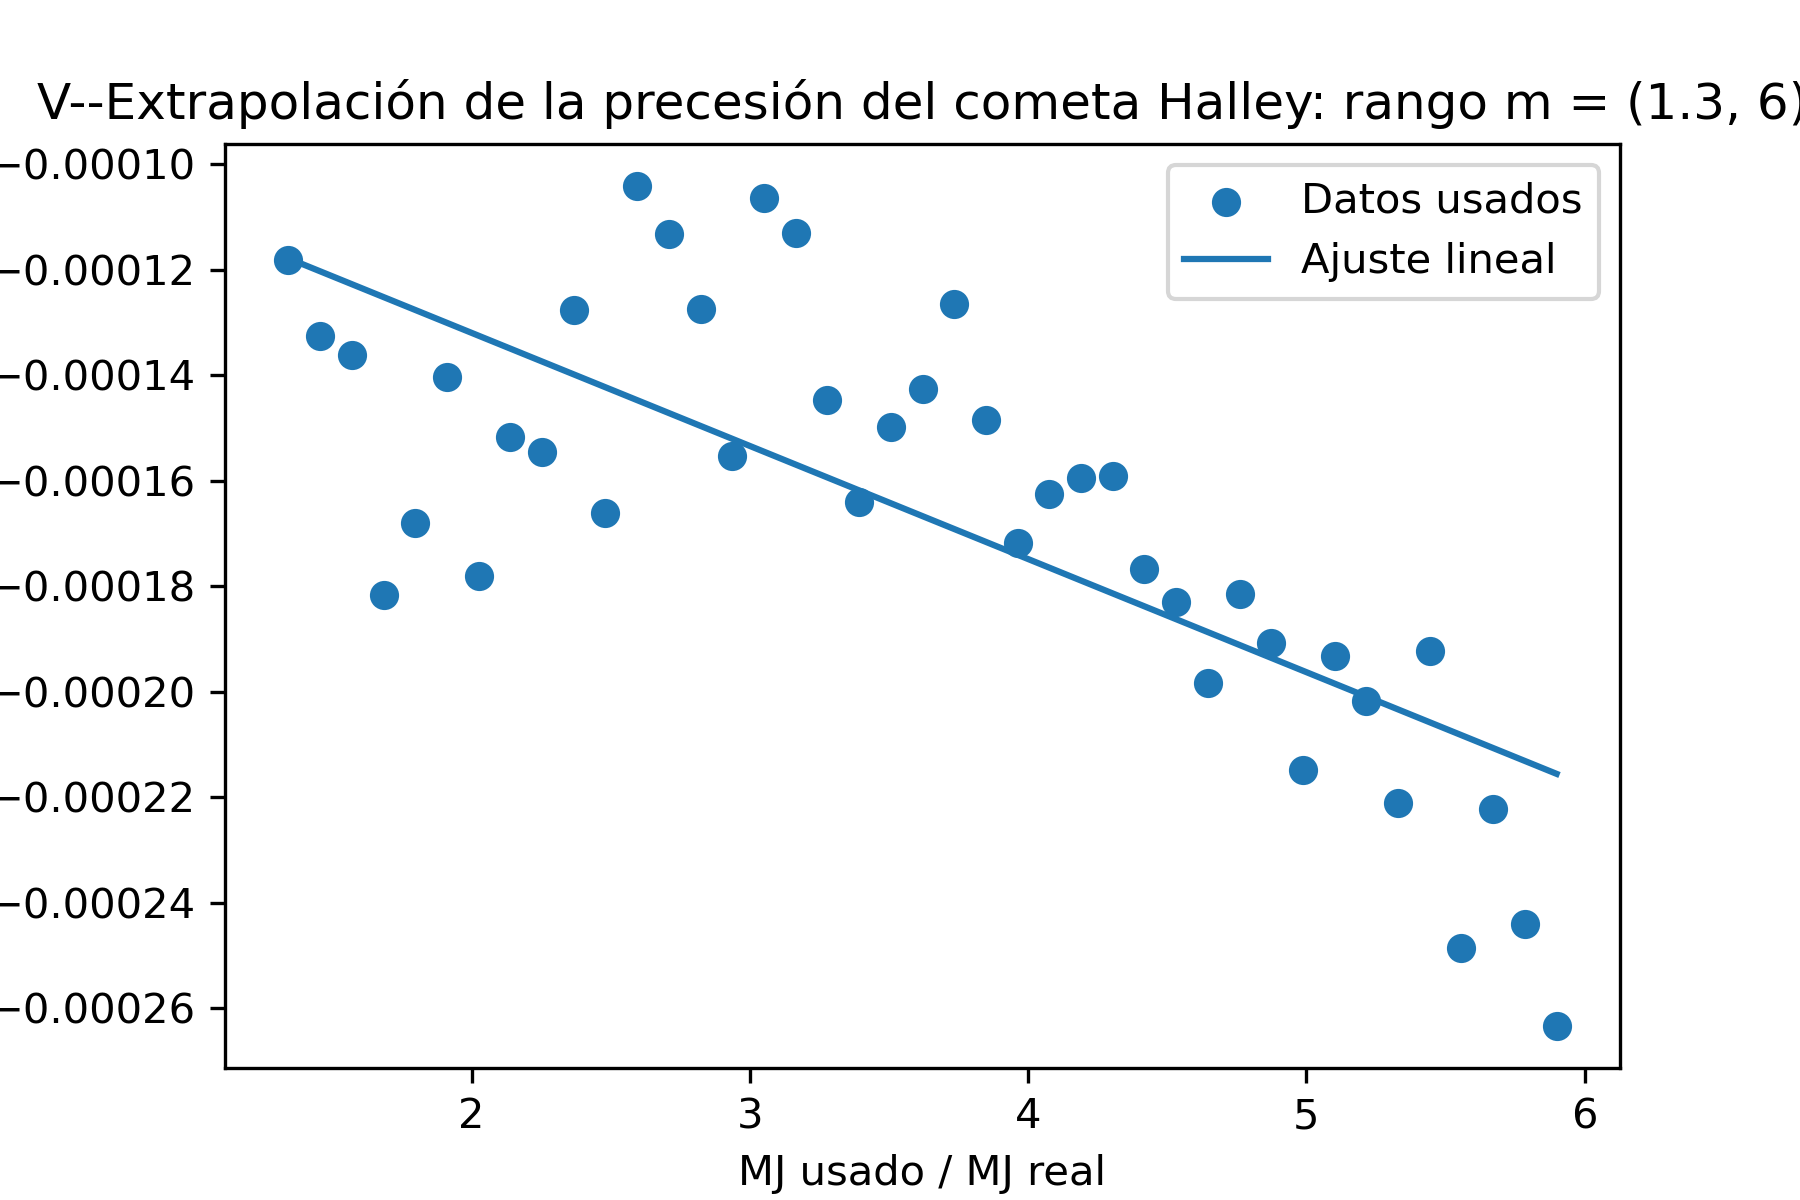
\includegraphics[width=\linewidth]{imagenes/prec_halley_rango_v.png}
    \caption{$\frac{M_{J,usada}}{M_{J,real}} \in (1.3, 6)$}
\end{subfigure}

\caption{Precesión del perihelio de Halley utilizando Verlet}
\label{fig:comparacion}
\end{figure}



La extrapolación lineal permite estimar la precesión real correspondiente a la masa verdadera de Júpiter. Se utiliza un filtrado de los resultados para descartar los datos más alejados de la tendencia general. 

Además, se excluyen del rango en ambos casos los valores muy cercanos a la masa de Júpiter real debido a que son considerablemente inestables y los datos cuya masa al menos 6 veces superior a la real.

Comparando los resultados de ambas simulaciones tras los filtrados se obtiene lo siguiente:
\begin{table}[H]
\centering
\begin{tabular}{|c|ccc|c|c|}
\hline
 & \multicolumn{3}{c|}{Precesión} &  &  \\ 
\cline{2-4}
Método & $rad/año$ & $arcseg/siglo$ & º/siglo & Pendiente (fit) & Ordenada (fit) \\ 
\hline
EC & $-1.08\cdot 10^{-4}$ & $-2.23\cdot 10^3$ & $-0.618$ & $-2.25\cdot 10^{-5}$ & $-8.54\cdot 10^{-5}$ \\ 
\hline
Verlet & $-1.11\cdot 10^{-4}$ & $-2.28\cdot 10^3$ & $-0.633$ & $-2.14\cdot 10^{-5}$ & $-8.91\cdot 10^{-5}$ \\ 
\hline
\end{tabular}
\caption{Comparación de los resultados de precesión y sus ajustes para los métodos iterativos empleados.}
\label{tab:ejemplo}
\end{table}

Tanto el resultado de precesión como los resultados de los ajustes salen similares en ambos métodos, aunque esta semejanza no es suficiente para sobreponerse a la aleatoriedad de los resultados de los ajustes. 

Se ha optado por la extrapolación de la precesión en función de una masa de Júpiter amplificada porque si aminoramos su masa, la precesión se vuelve difícilmente detectable y, cuando utilizamos la masa real, los resultados de la precesión dependen fuertemente de las condiciones numéricas de la simulación.

No obstante, esta tendencia rectilínea de la precesión en función del factor multiplicativo no es una tendencia global, sino local. Muestra de esto es el valor de la ordenada en el origen, la cual no es 0, pese a que si la masa de Júpiter fuera nula no habría precesión.

Por estos motivos (y por las complejidades físicas propias del cometa Halley que no hemos tenido en cuenta en este primer acercamiento), el resultado de la precesión del orden de 0.6 º/siglo es únicamente válido como una estimación inicial y requeriría de métodos más estables y precisos para obtener el resultado exacto.

\subsection{Caso de Mercurio}

Se realizaron una serie de simulaciones adicionales para Mercurio incluyendo la únicamente la perturbación de Júpiter y extrapolando el resultado para diferentes masas.

\begin{figure}[H]
\centering
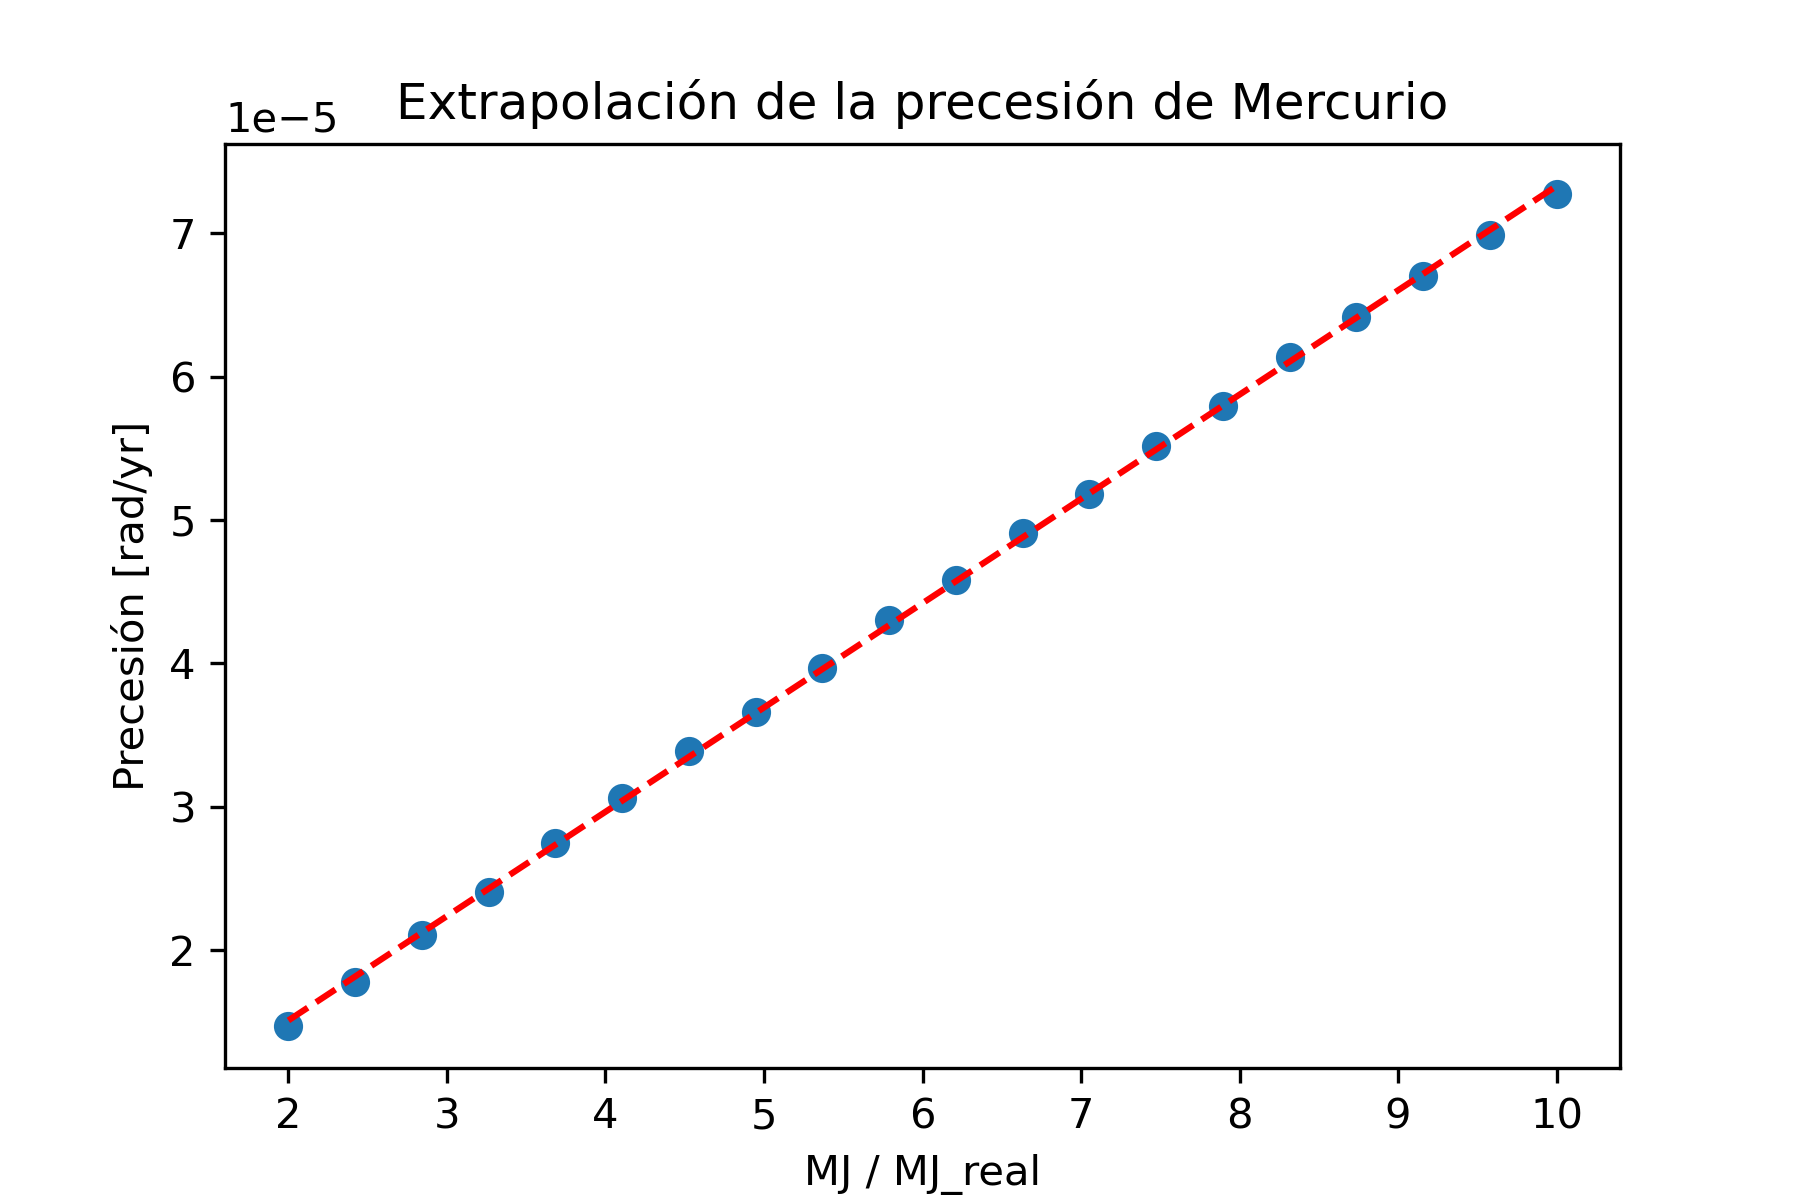
\includegraphics[width=0.8\textwidth]{imagenes/prec_mercurio_v.png}
\caption{Extrapolación de la precesión de Mercurio.}
\end{figure}

Se puede realizar la misma tabla que se creó para el cometa Halley:

\begin{table}[H]
\centering
\begin{tabular}{|c|c|c|}
\hline
Método & Precesión extrapolada (arcseg/siglo) & Ordenada (arcseg/siglo) \\ 
\hline
Verlet & $162.1$ & $12.1$  \\ 
\hline
\end{tabular}
\caption{Resultados de la extrapolación de la precesión de Mercurio.}
\label{tab:mercurio}
\end{table}

El resultado que predice la mecánica newtoniana para la precesión provocada por Júpiter a la órbita de Mercurio es de 153.6 arcseg/siglo \ref{bambi}. Mediante el método de extrapolación se obtiene que la precesión es de 162.1, una diferencia menor que el 10 \% del valor real.

Por otro lado, como los resultados de la precesión de Mercurio son bastante estables (al contrario que los obtenidos con el cometa Halley), se puede realizar directamente el caso en el que la masa de Júpiter es la real y se obtiene una precesión de 151.6 arcseg/siglo, un resultado con un margen de error cercano al 1\%.

No obstante, los resultados de estas simulaciones no son completamente fiables debido a que si directamente suponemos que Júpiter no tiene masa, se obtiene una precesión de -2.5 arcseg/siglo y si extrapolamos hasta MJ=0 obtenemos que la precesión es de 12.5 arcseg/siglo. Estos valores deberían de ser ambos 0 pero debido a la incertidumbre propia de los métodos numéricos (dt), los resultados simulados se alejan ligeramente de la realidad.

Aún con estas discrepancias, el método de verlet parece ser una forma fiable de realizar una primera estimación del valor de la precesión de los cuerpos celestes.

\section{Conclusiones}

En este trabajo se ha desarrollado una simulación numérica del movimiento orbital del cometa Halley utilizando métodos de integración temporal discretos.

Los resultados obtenidos permiten reproducir correctamente las principales características dinámicas de su órbita, incluyendo su elevada excentricidad y la variación de velocidad a lo largo de la trayectoria.

Asimismo, se ha analizado la conservación de la energía y el momento angular, verificando la estabilidad del método numérico empleado.

La introducción de la perturbación gravitatoria de Júpiter permite observar la precesión de la órbita del cometa que puede cuantificarse mediante técnicas de extrapolación, debido a la inestabilidad del método para valores de la masa de Júpiter cercanos al real.

Además, se han verificado las predicciones realizadas por la dinámica newtoniana para la órbita de Mercurio debido a la presencia de Júpiter.

Estos resultados ilustran cómo simulaciones numéricas relativamente sencillas pueden servir para obtener una estimación de la dinámica orbital en el sistema solar.

\begin{thebibliography}{9}

\bibitem{giordano}
N. J. Giordano and H. Nakanishi,
\textit{Computational Physics},
2nd ed., Pearson Prentice Hall, 2006.
\label{giordano}
\bibitem{bambi2018}
C. Bambi,
\textit{Introduction to General Relativity: A Course for Undergraduate Students of Physics},
Undergraduate Lecture Notes in Physics,
Springer Nature Singapore Pte Ltd., 2018.
\label{bambi}


\end{thebibliography}

\newpage
\appendix
\section*{Anexo A: Variables empleadas}

\begin{center}
\begin{tabular}{ll}
\hline
Variable & Significado \\
\hline
$GMS$ & Producto $GM_{\odot}$ \\
$m$ & Masa \\
$x,y$ & Posición del cometa \\
$vx,vy$ & Velocidad del cometa \\
$r$ & Distancia al Sol \\
$v^2$ & Velocidad al cuadrado \\
$E_c$ & Energía cinética \\
$E_p$ & Energía potencial \\
$E_t$ & Energía total \\
$L$ & Momento angular \\
$x_j,y_j$ & Posición de Júpiter \\
$vx_j,vy_j$ & Velocidad de Júpiter \\
$MJ$ & Masa de Júpiter \\
$dt$ & Paso temporal \\
$T$ & Tiempo total de simulación \\
$a$ & Semieje mayor \\
$e$ & Excentricidad orbital \\
$r_p$ & Perihelio \\
$r_a$ & Afelio \\
\hline
\end{tabular}
\end{center}
\end{document}